\begin{figure}[H]
    \centering
    \begin{minipage}[t]{0.45\textwidth}
        \centering
        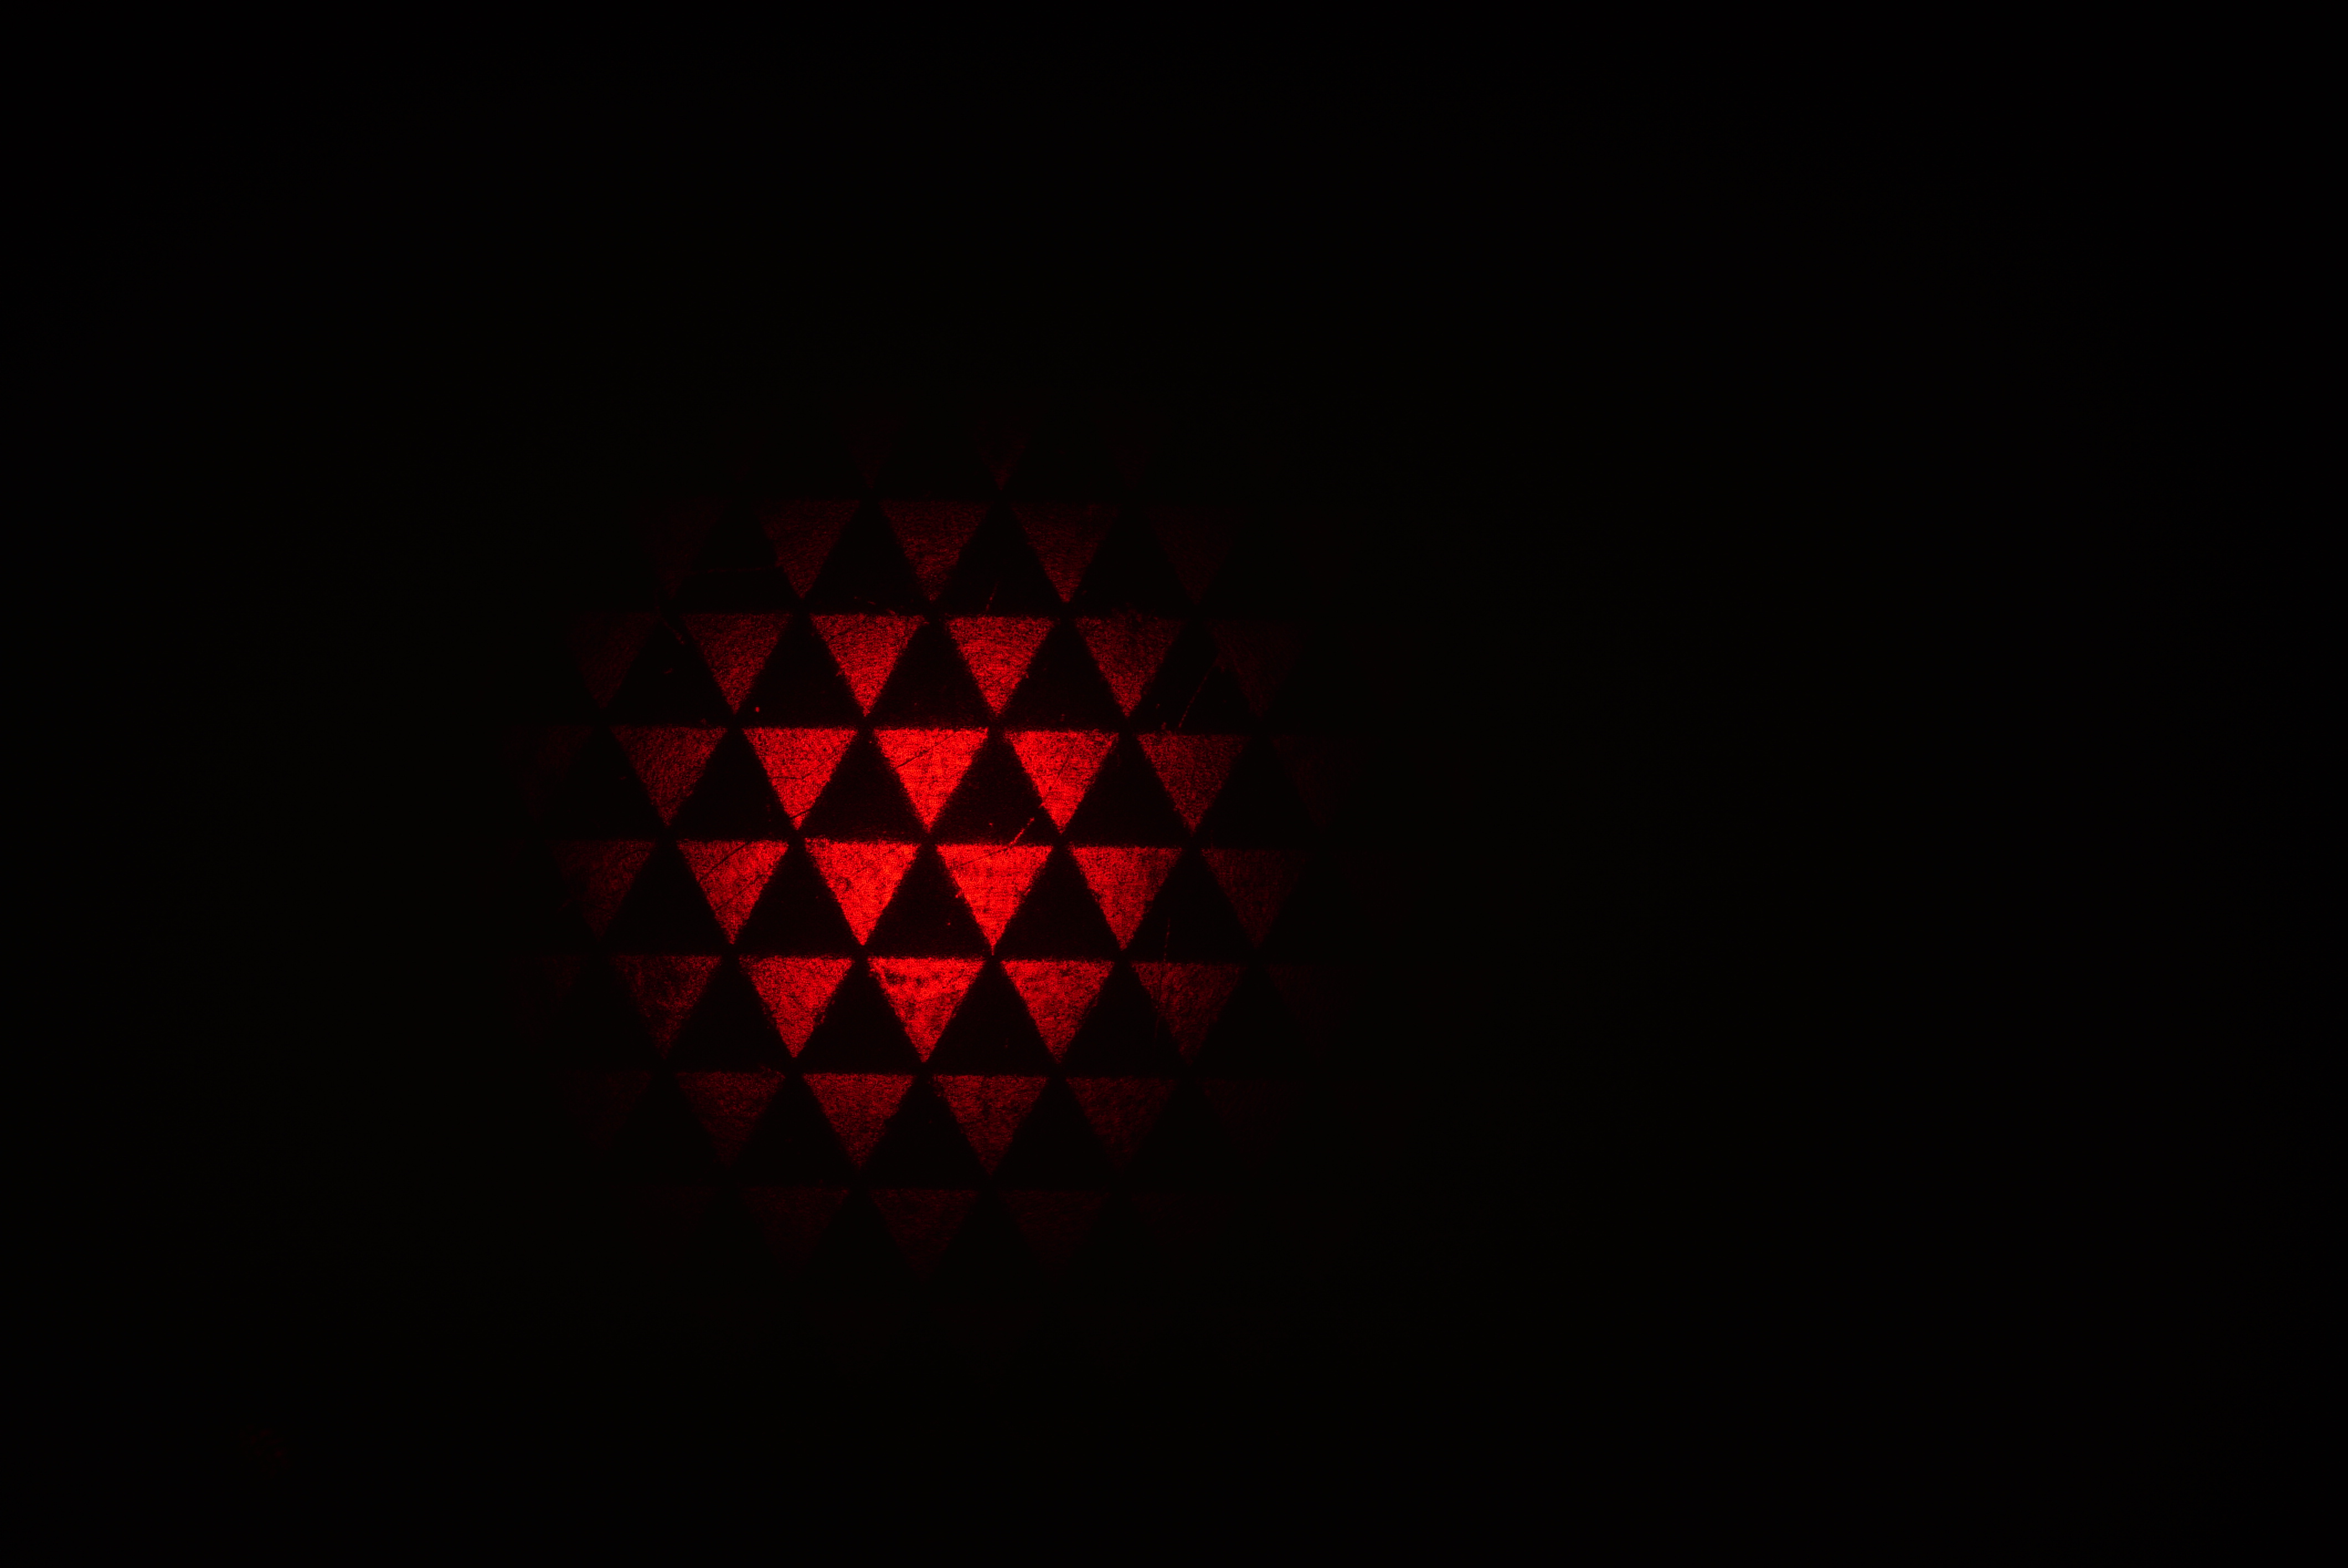
\includegraphics[ width = 0.95 \linewidth ]{figures/AperatureImages/DSC01549.JPG}
        \caption{The captured inverse Fourier transform using no aperture}
    \end{minipage}%
    \hspace{0.5cm}
    \begin{minipage}[t]{0.45\textwidth}
        \centering
        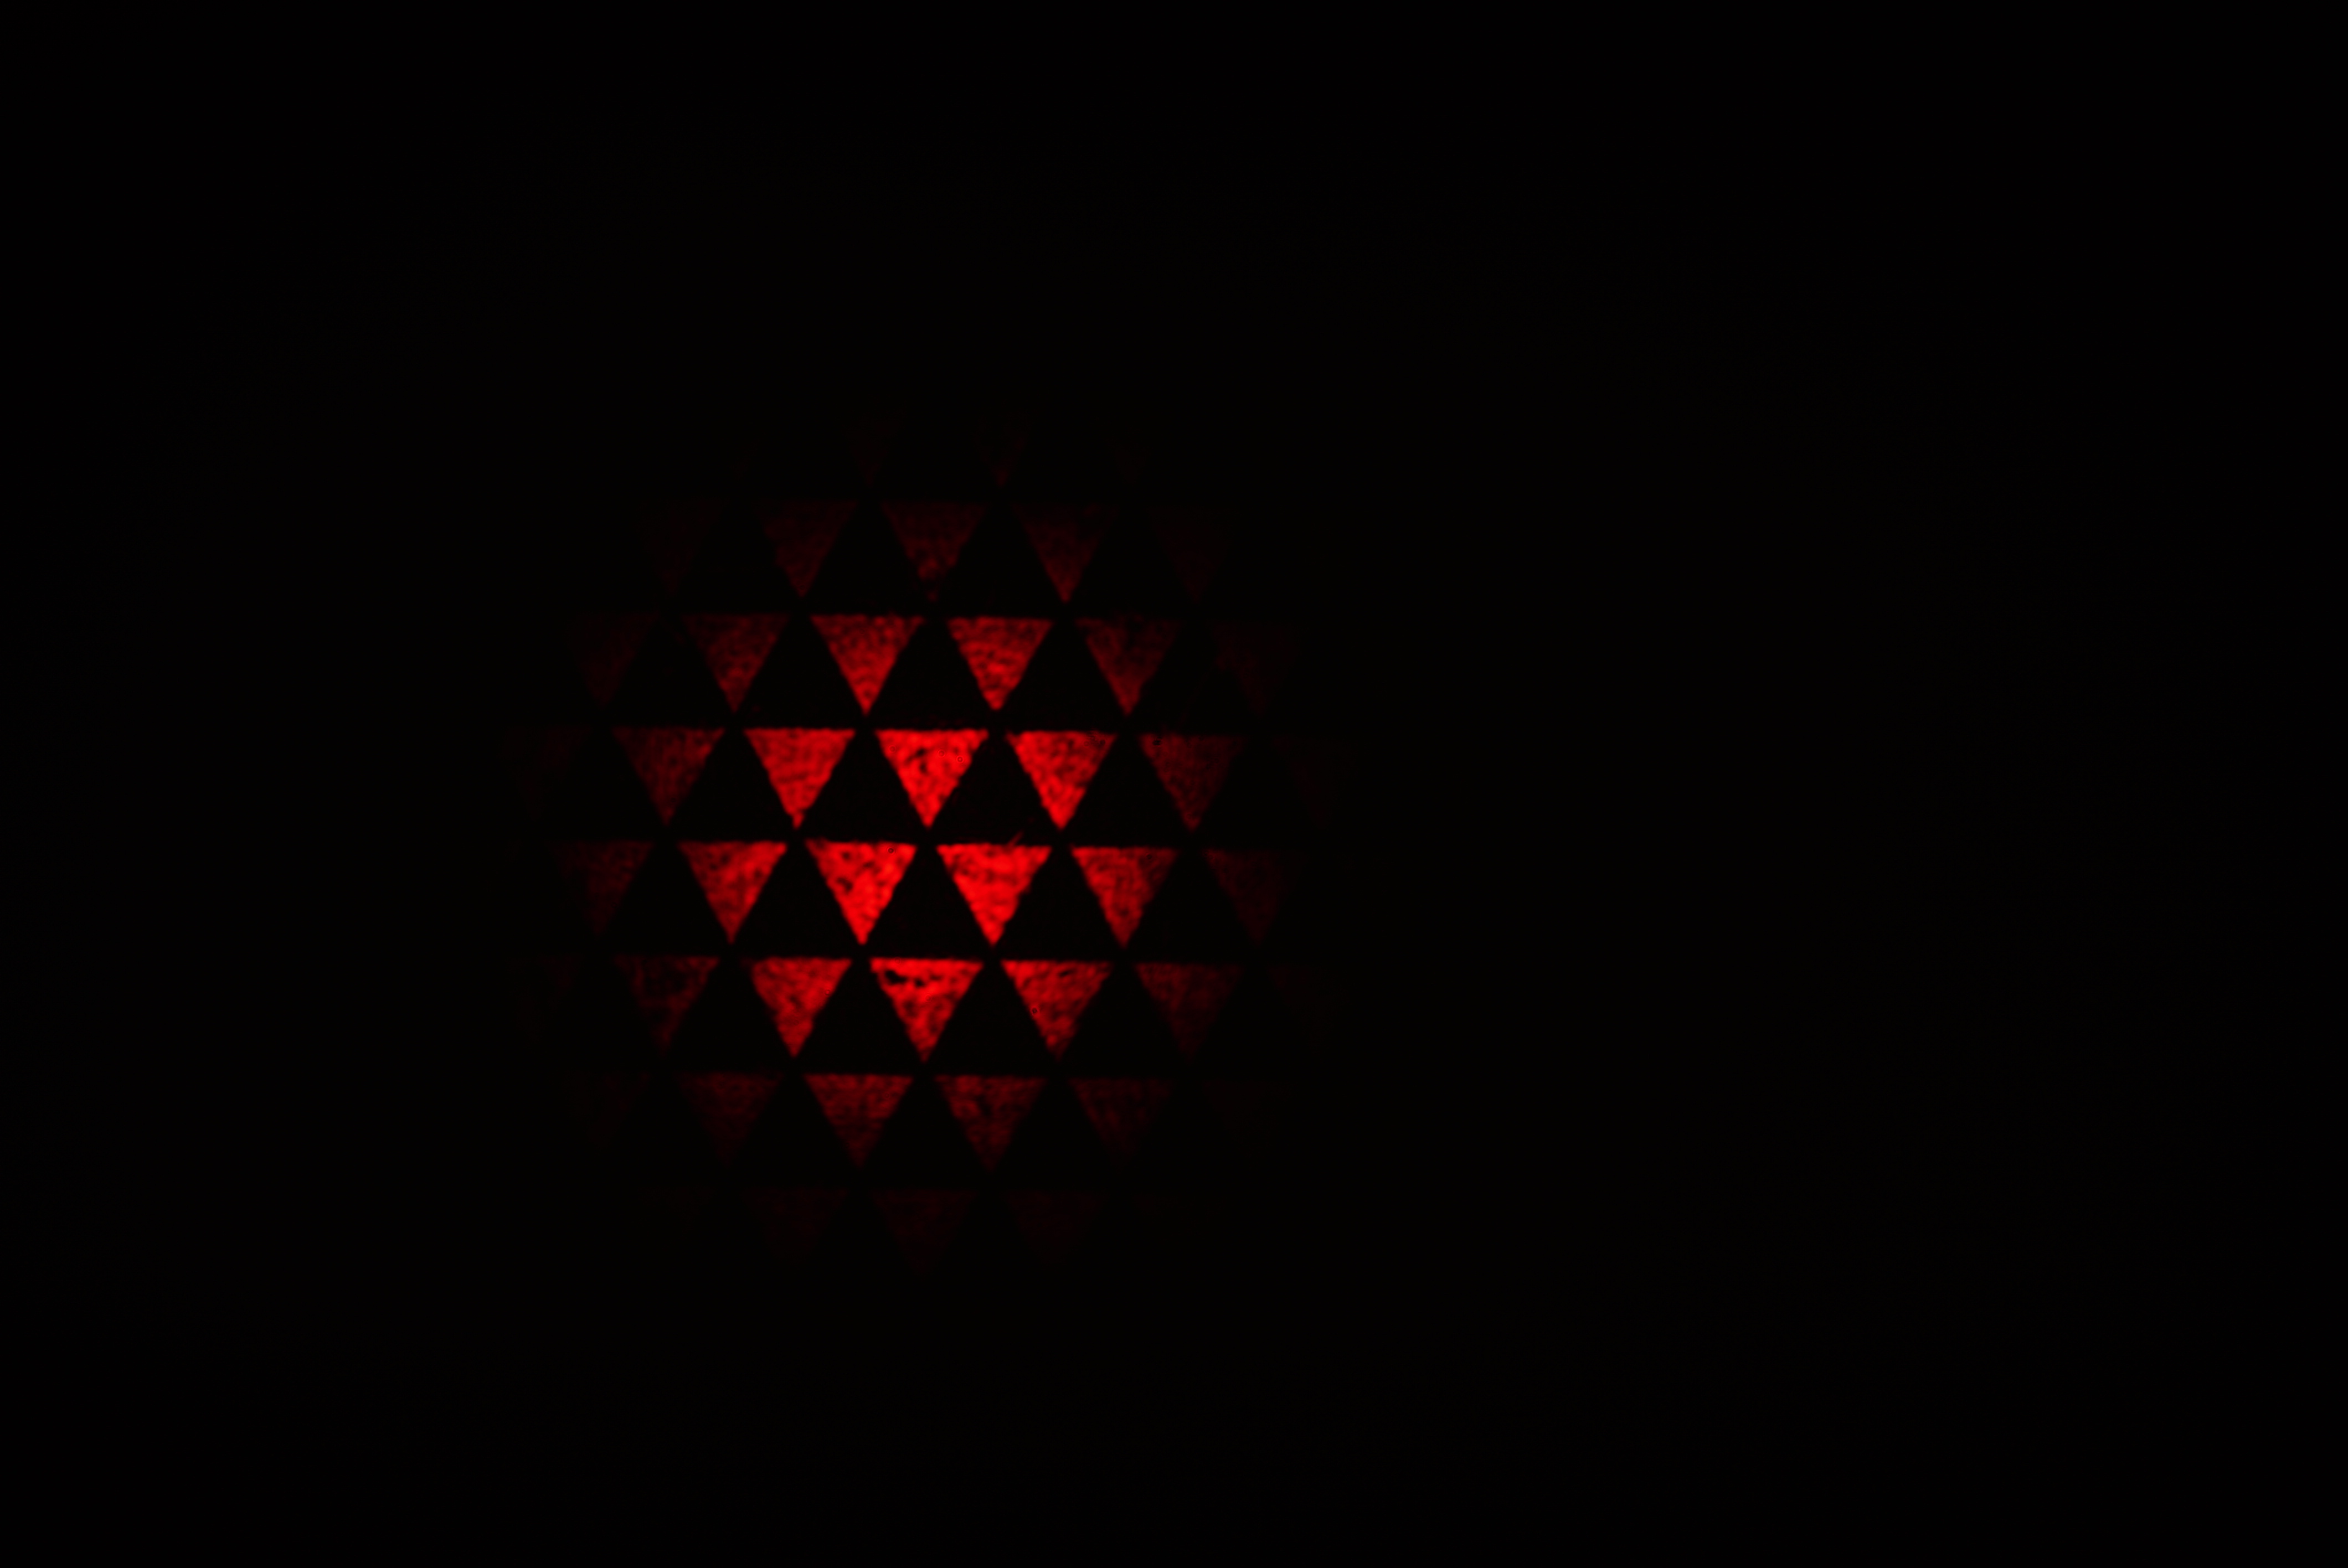
\includegraphics[ width = 0.95 \linewidth ]{figures/AperatureImages/DSC01548.JPG}
        \caption{The captured inverse Fourier transform using the aperture with a diameter of $2.0 \ \si{mm}$}
    \end{minipage}%
    \vspace{1.5cm}
    \begin{minipage}[t]{0.45\textwidth}
        \centering
        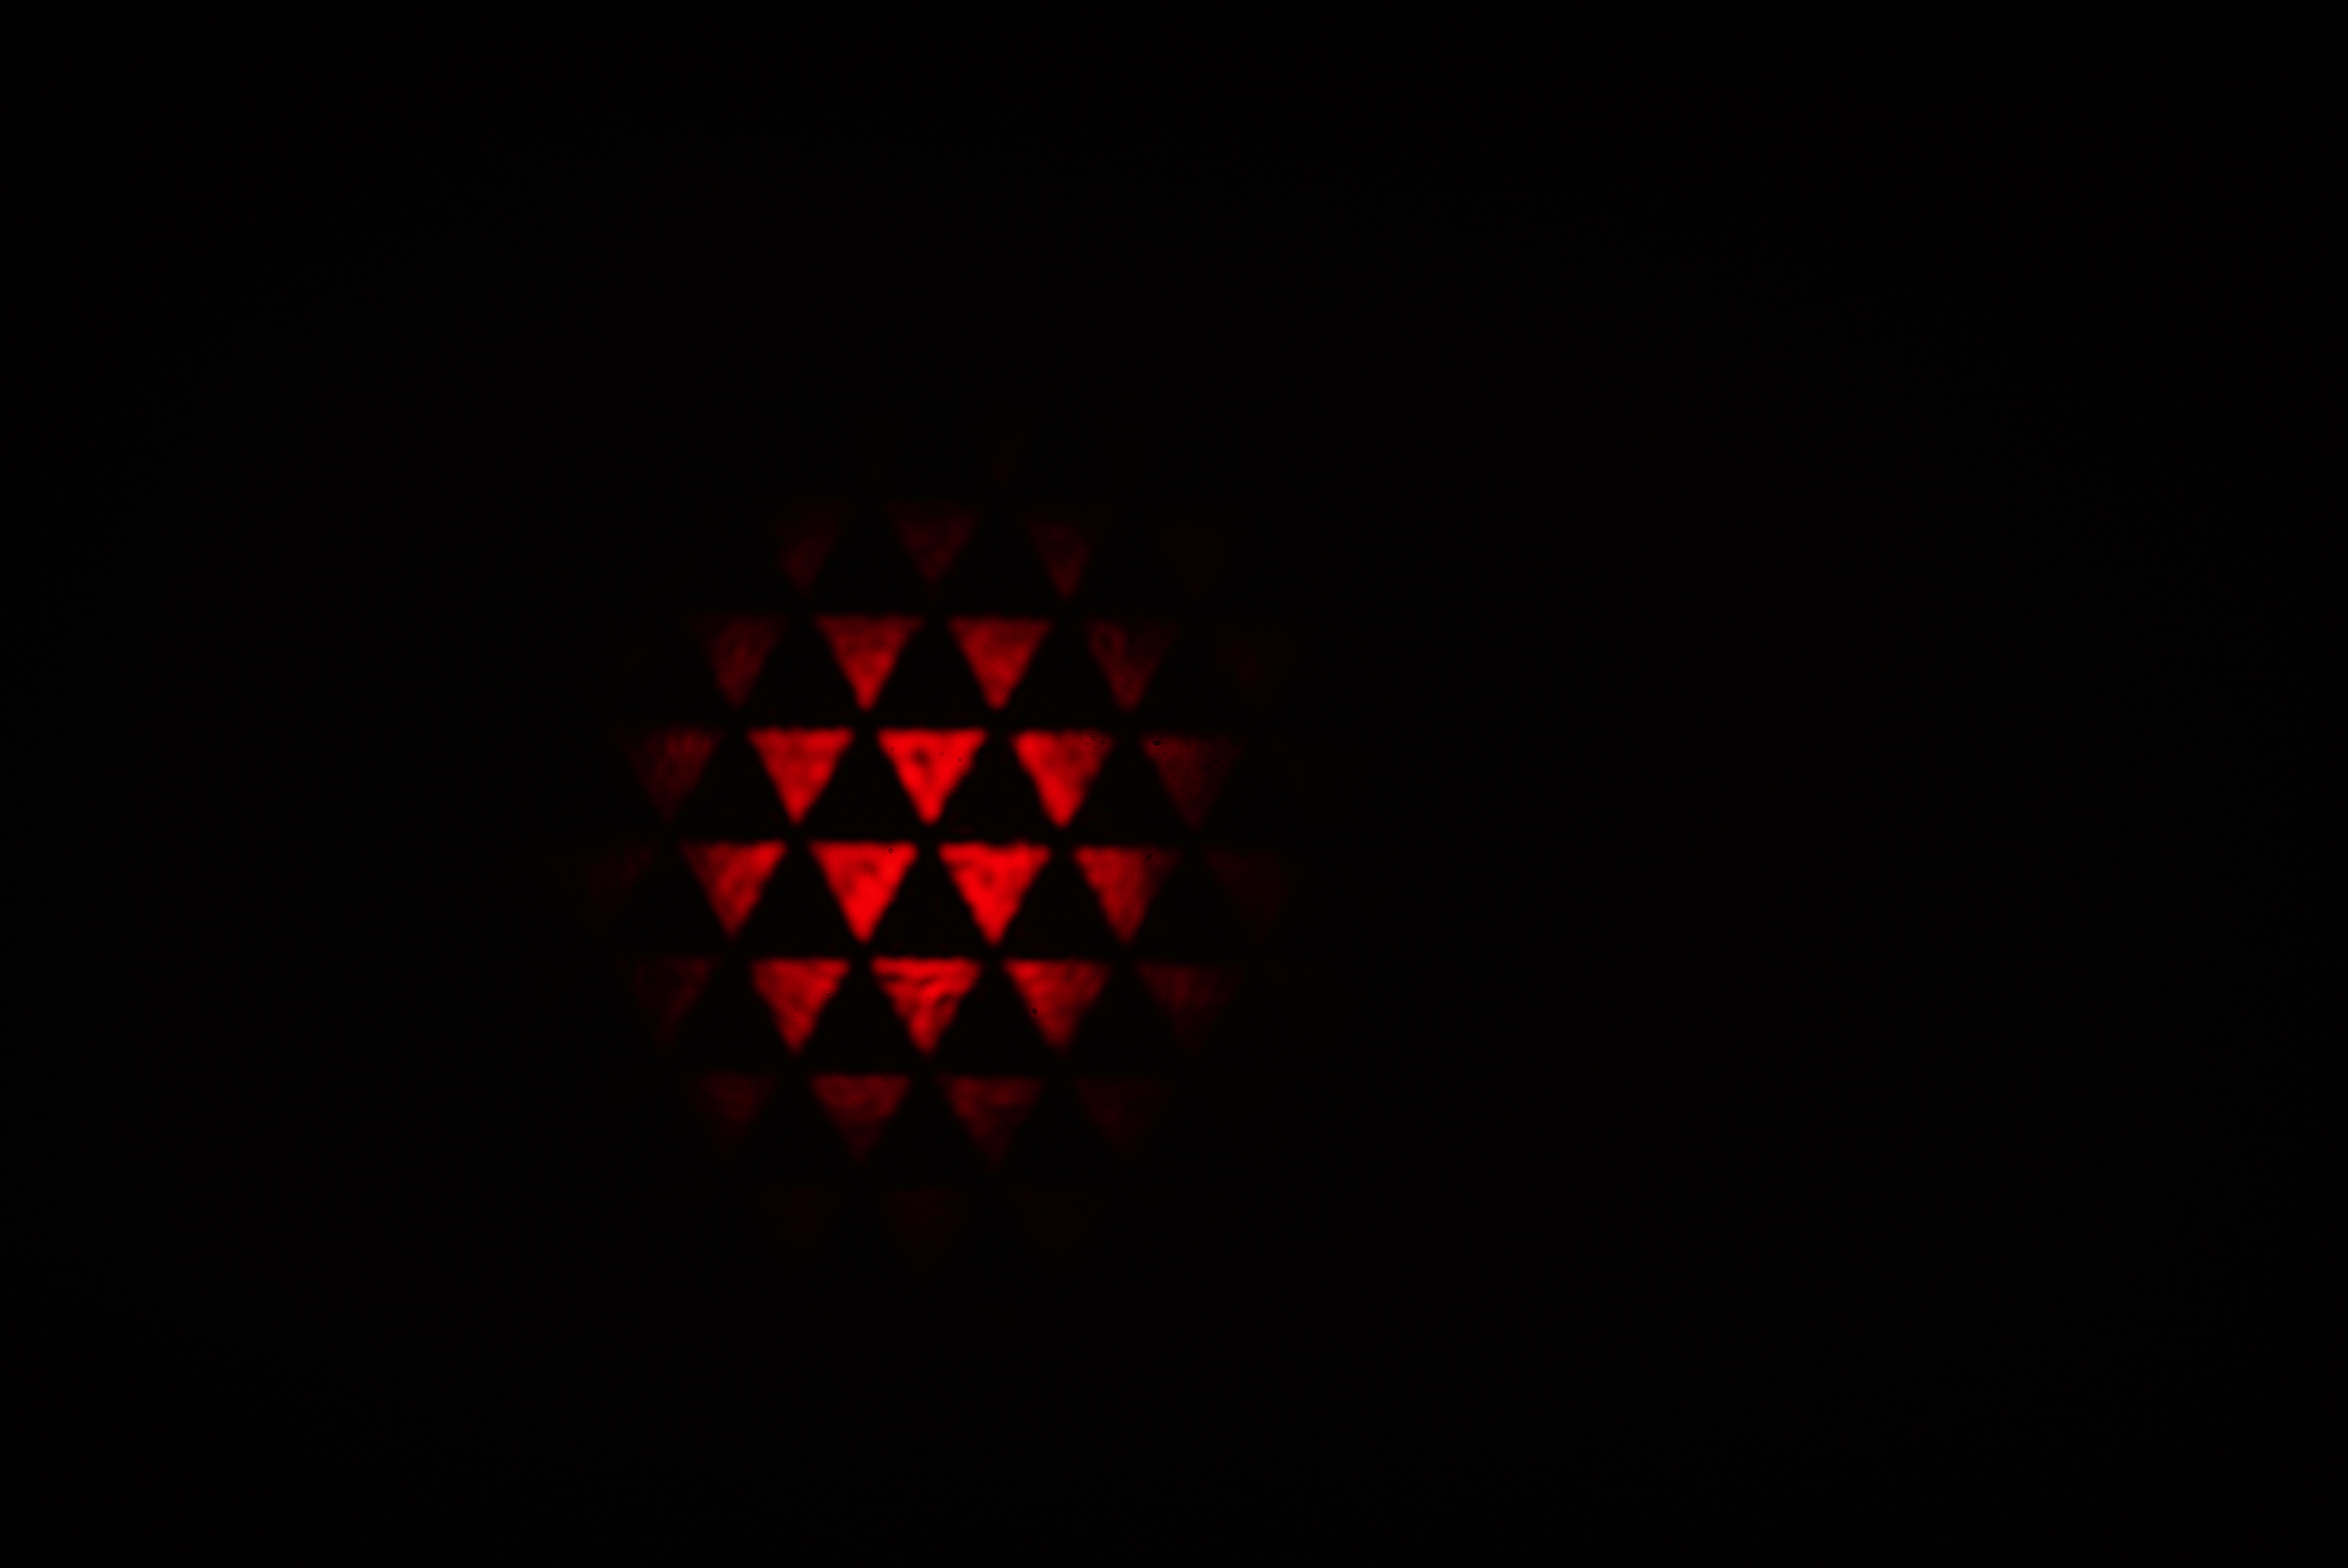
\includegraphics[ width = 0.95 \linewidth ]{figures/AperatureImages/DSC01547.JPG}
        \caption{The captured inverse Fourier transform using the aperture with a diameter of $1.0 \ \si{mm}$}
    \end{minipage}%
    \hspace{0.5cm}
    \begin{minipage}[t]{0.45\textwidth}
        \centering
        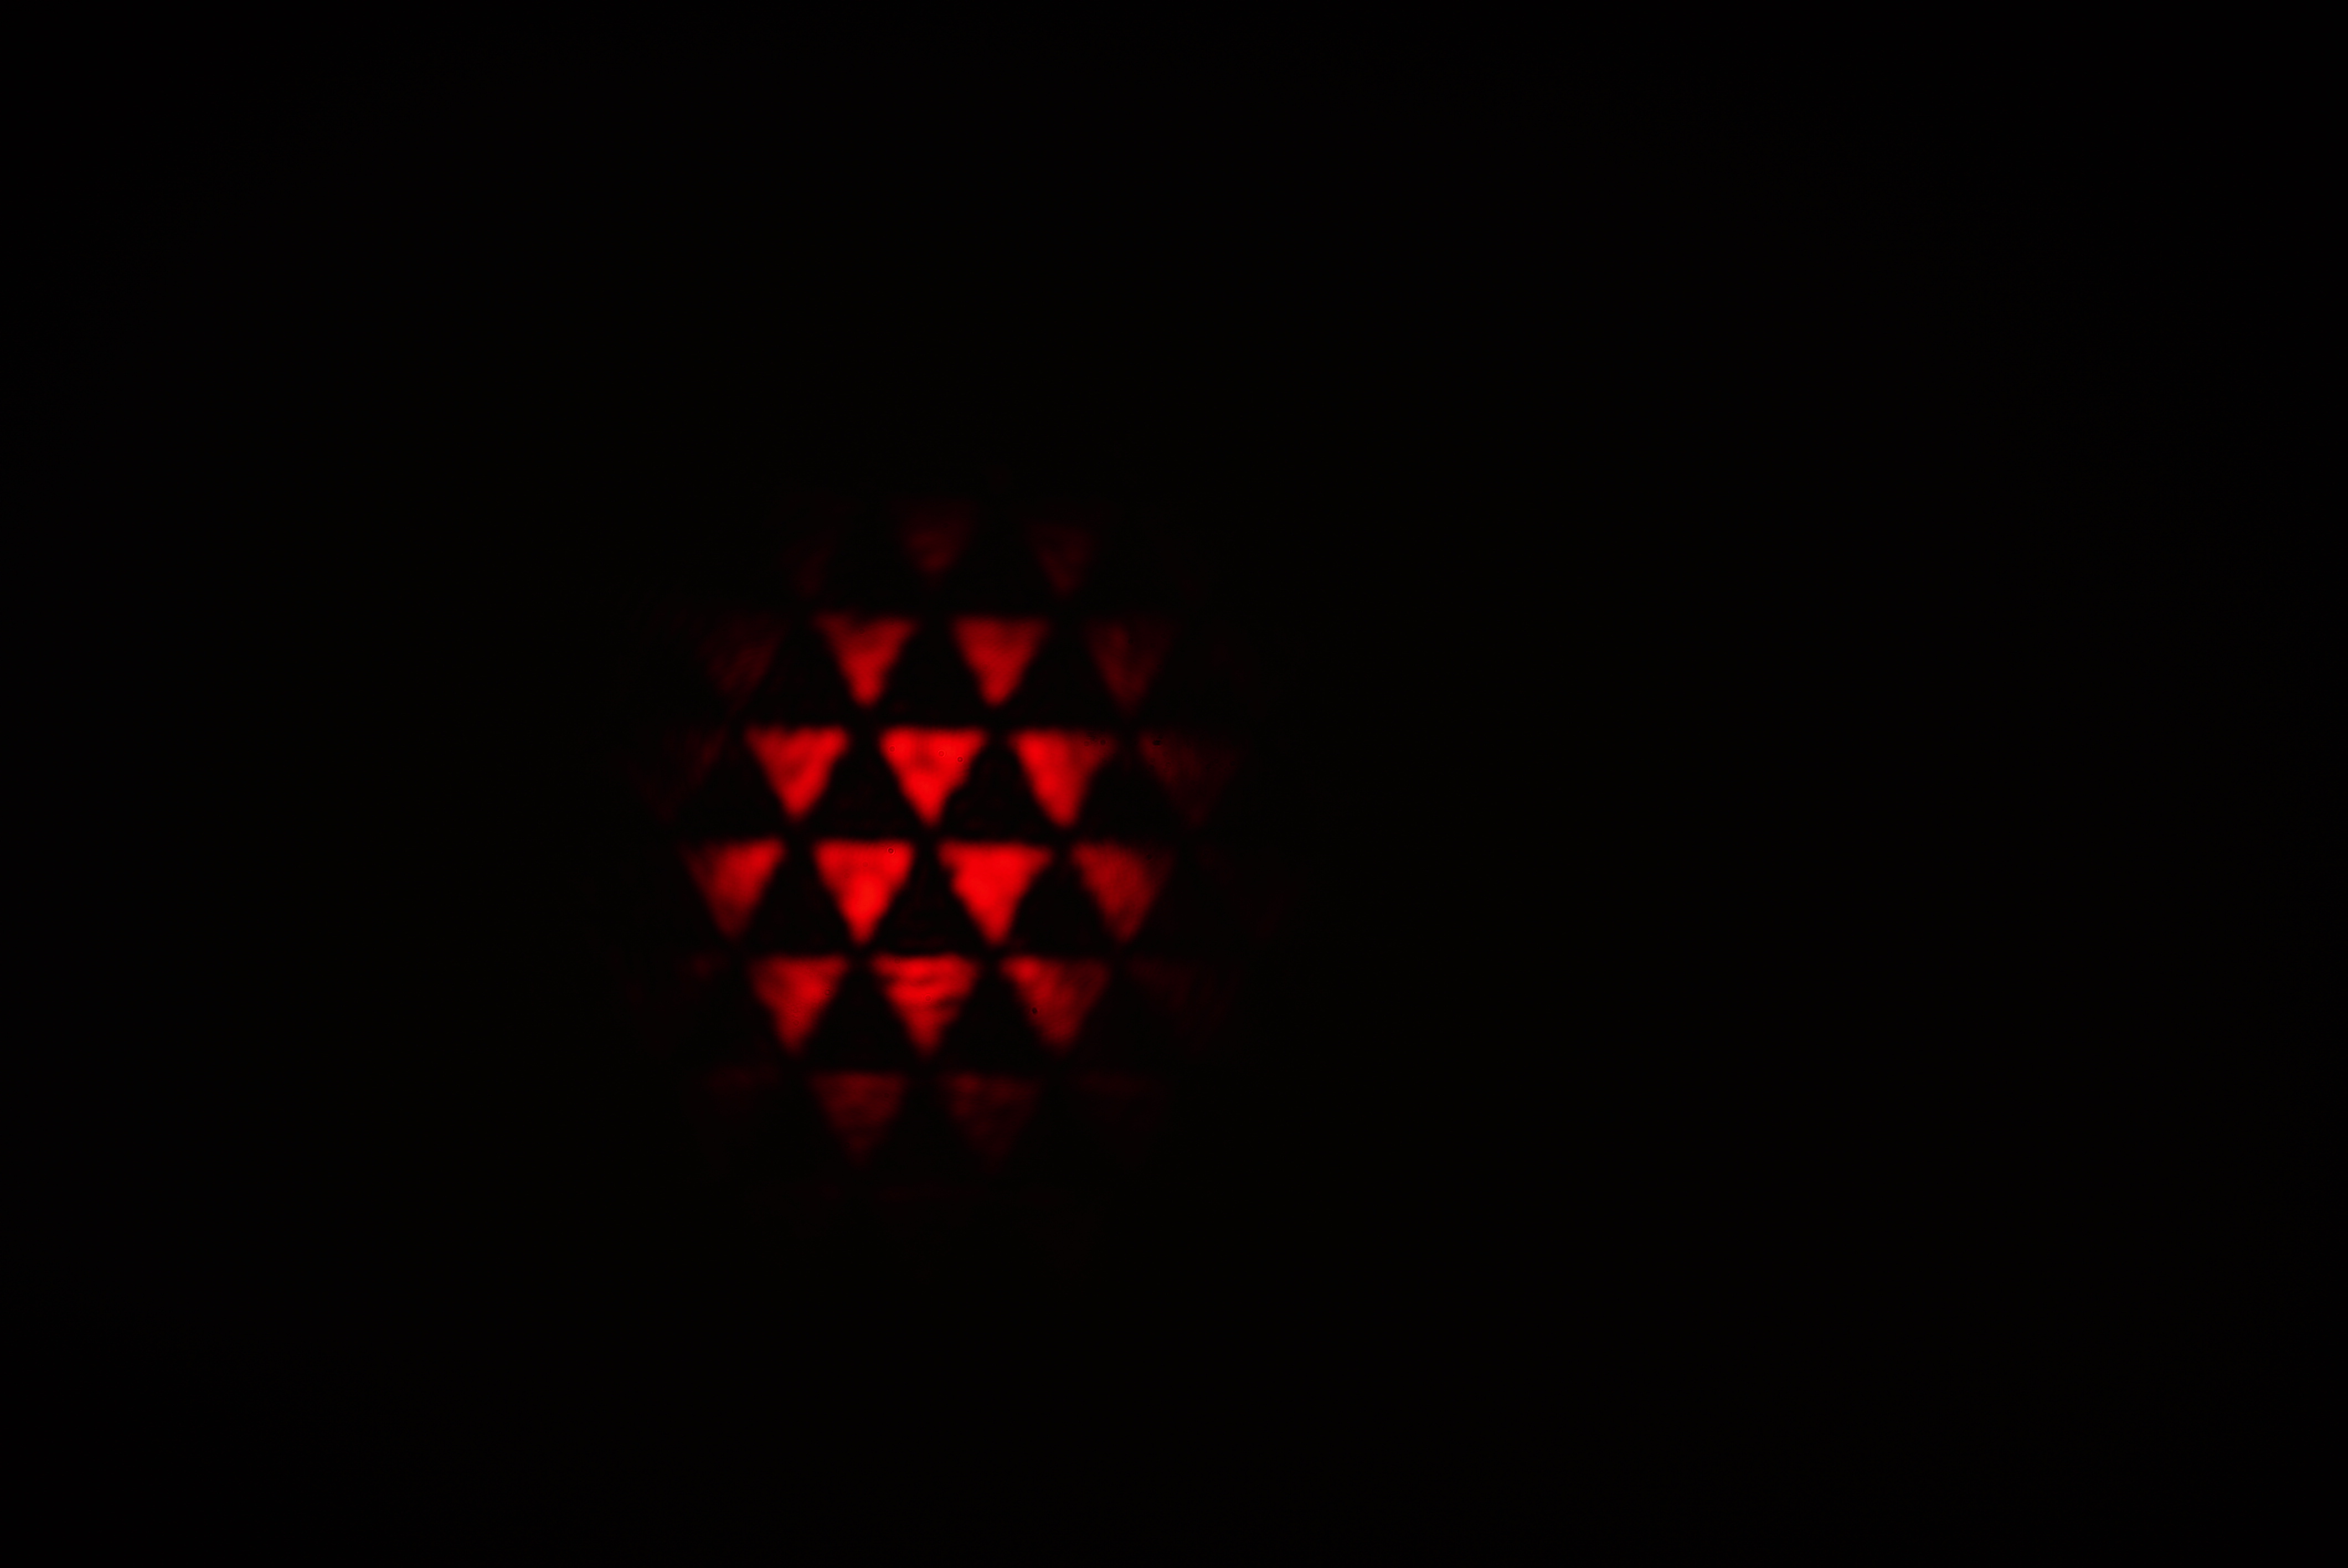
\includegraphics[ width = 0.95 \linewidth ]{figures/AperatureImages/DSC01546.JPG}
        \caption{The captured inverse Fourier transform using the aperture with a diameter of $0.70 \ \si{mm}$}
    \end{minipage}%
    \vspace{1.5cm}
    \begin{minipage}[t]{0.45\textwidth}
        \centering
        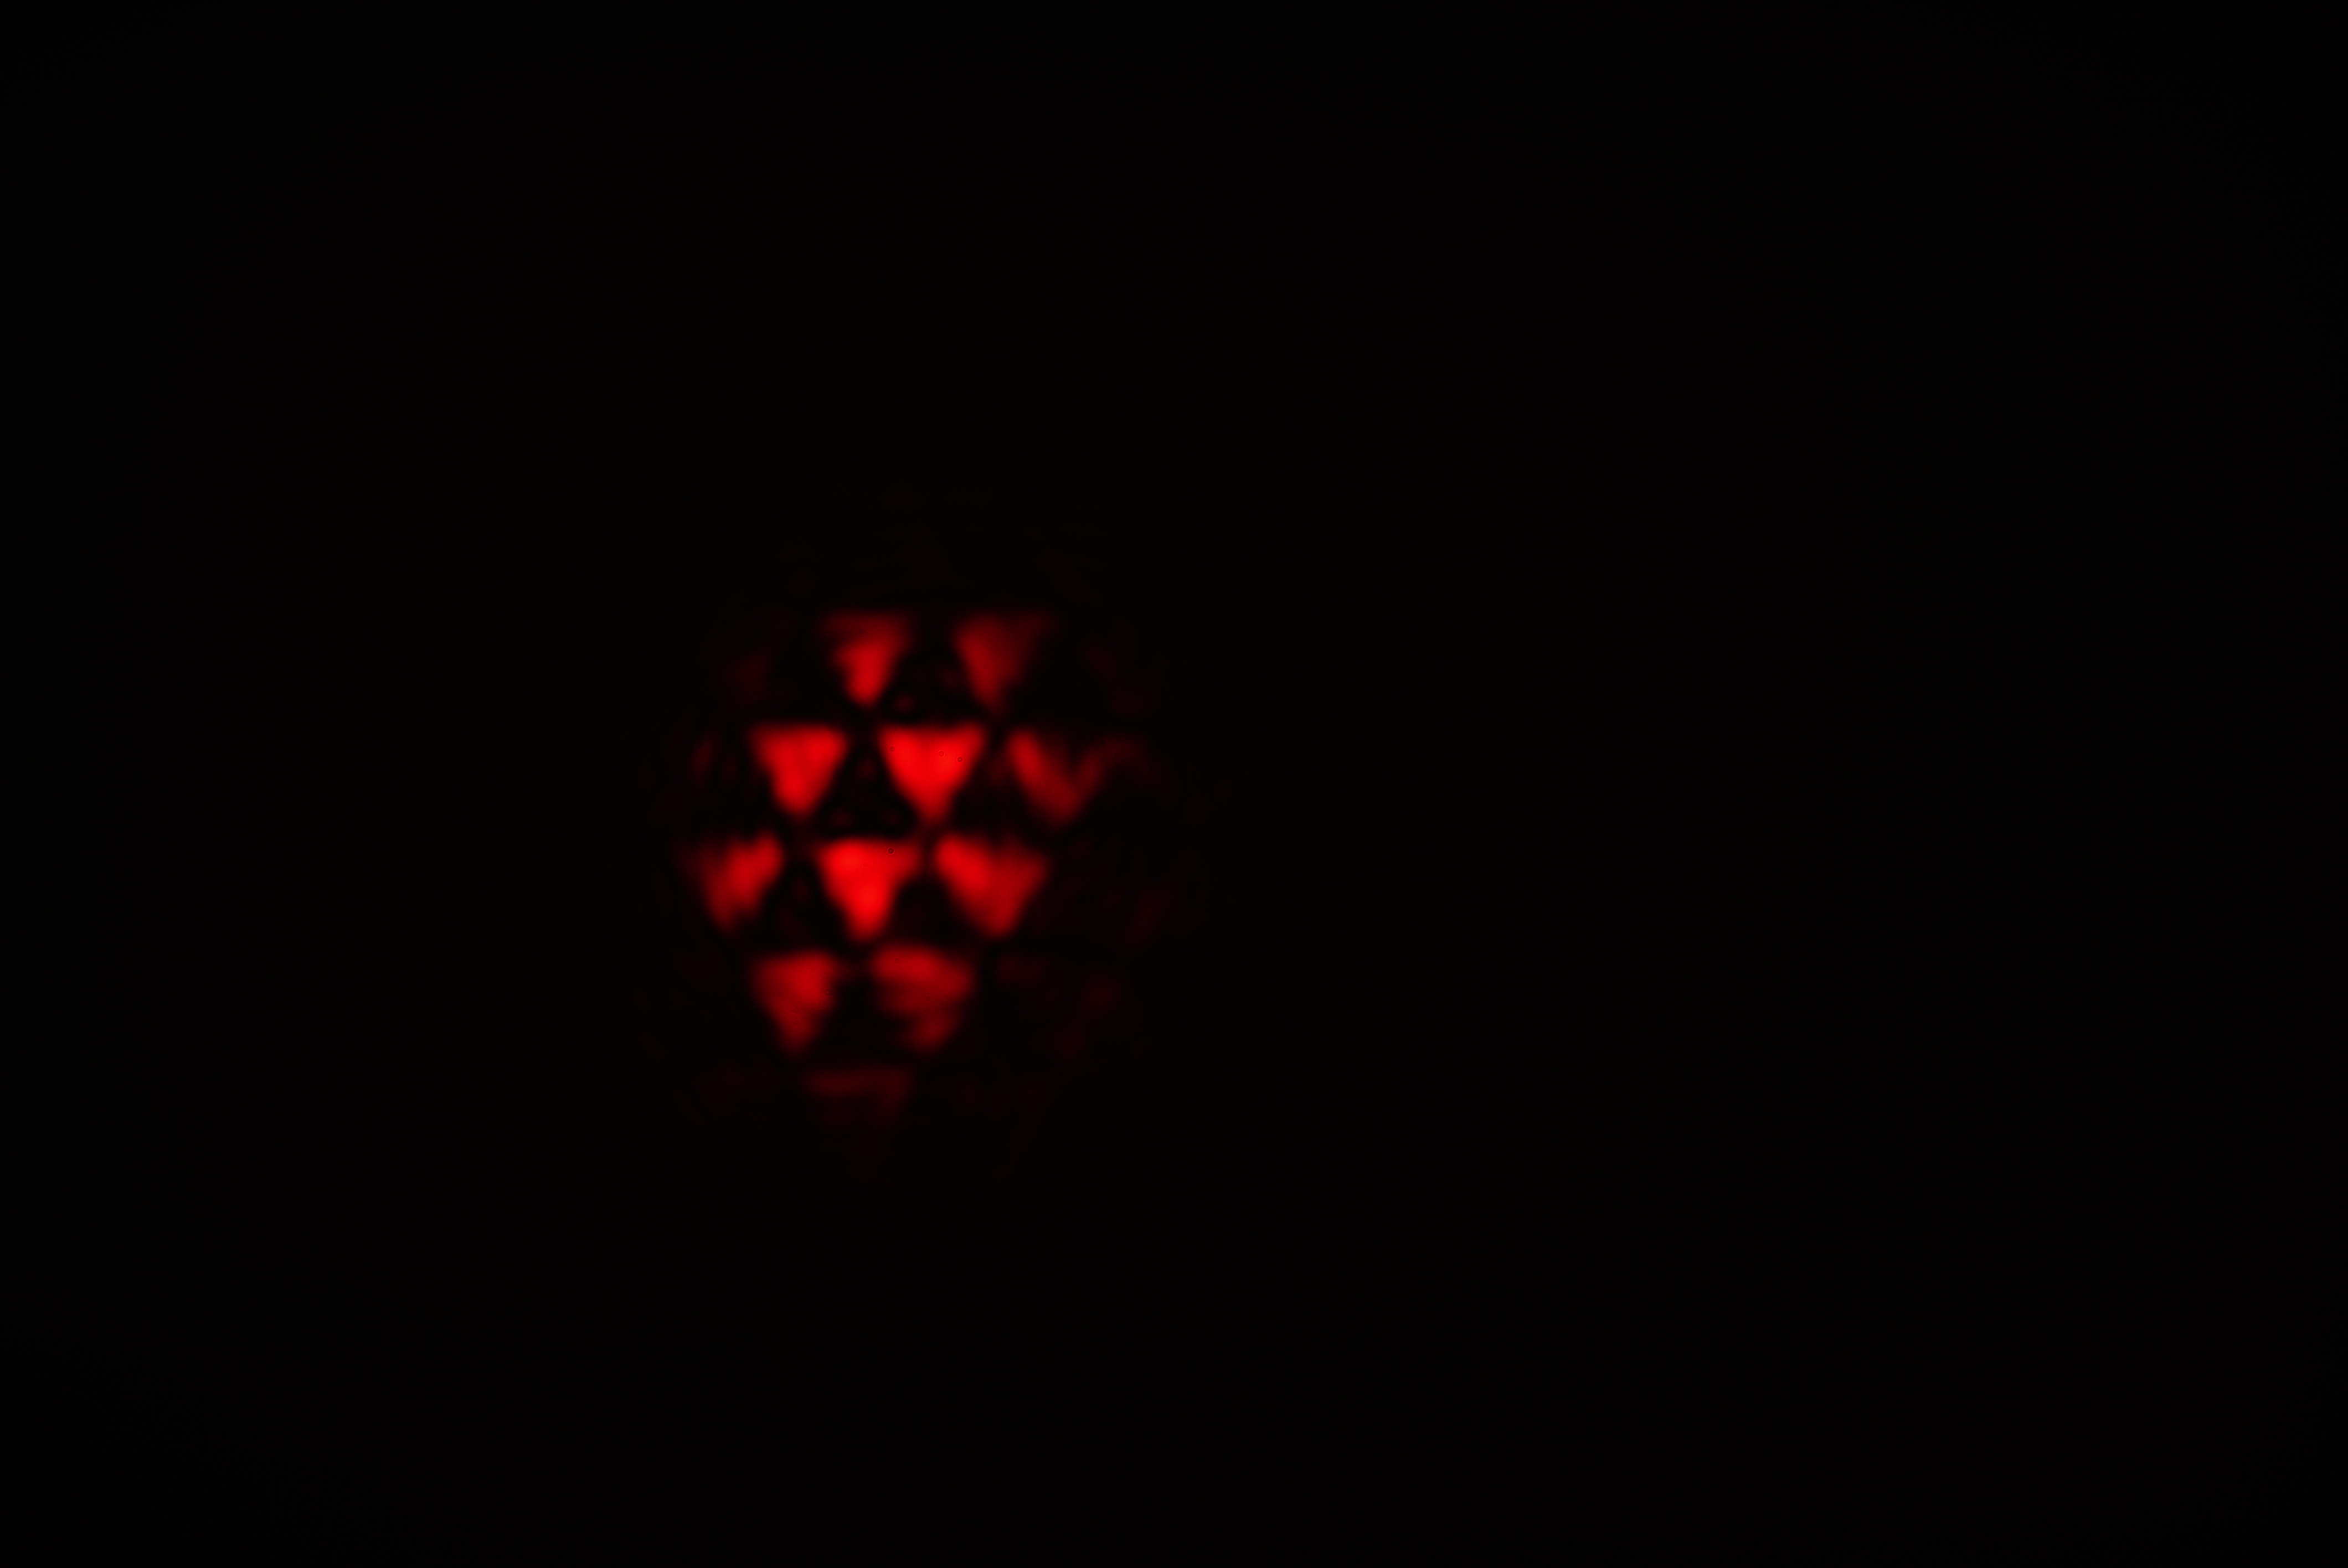
\includegraphics[ width = 0.95 \linewidth ]{figures/AperatureImages/DSC01545.JPG}
        \caption{The captured inverse Fourier transform using the aperture with a diameter of $0.50 \ \si{mm}$}
    \end{minipage}%
    \hspace{0.5cm}
    \begin{minipage}[t]{0.45\textwidth}
        \centering
        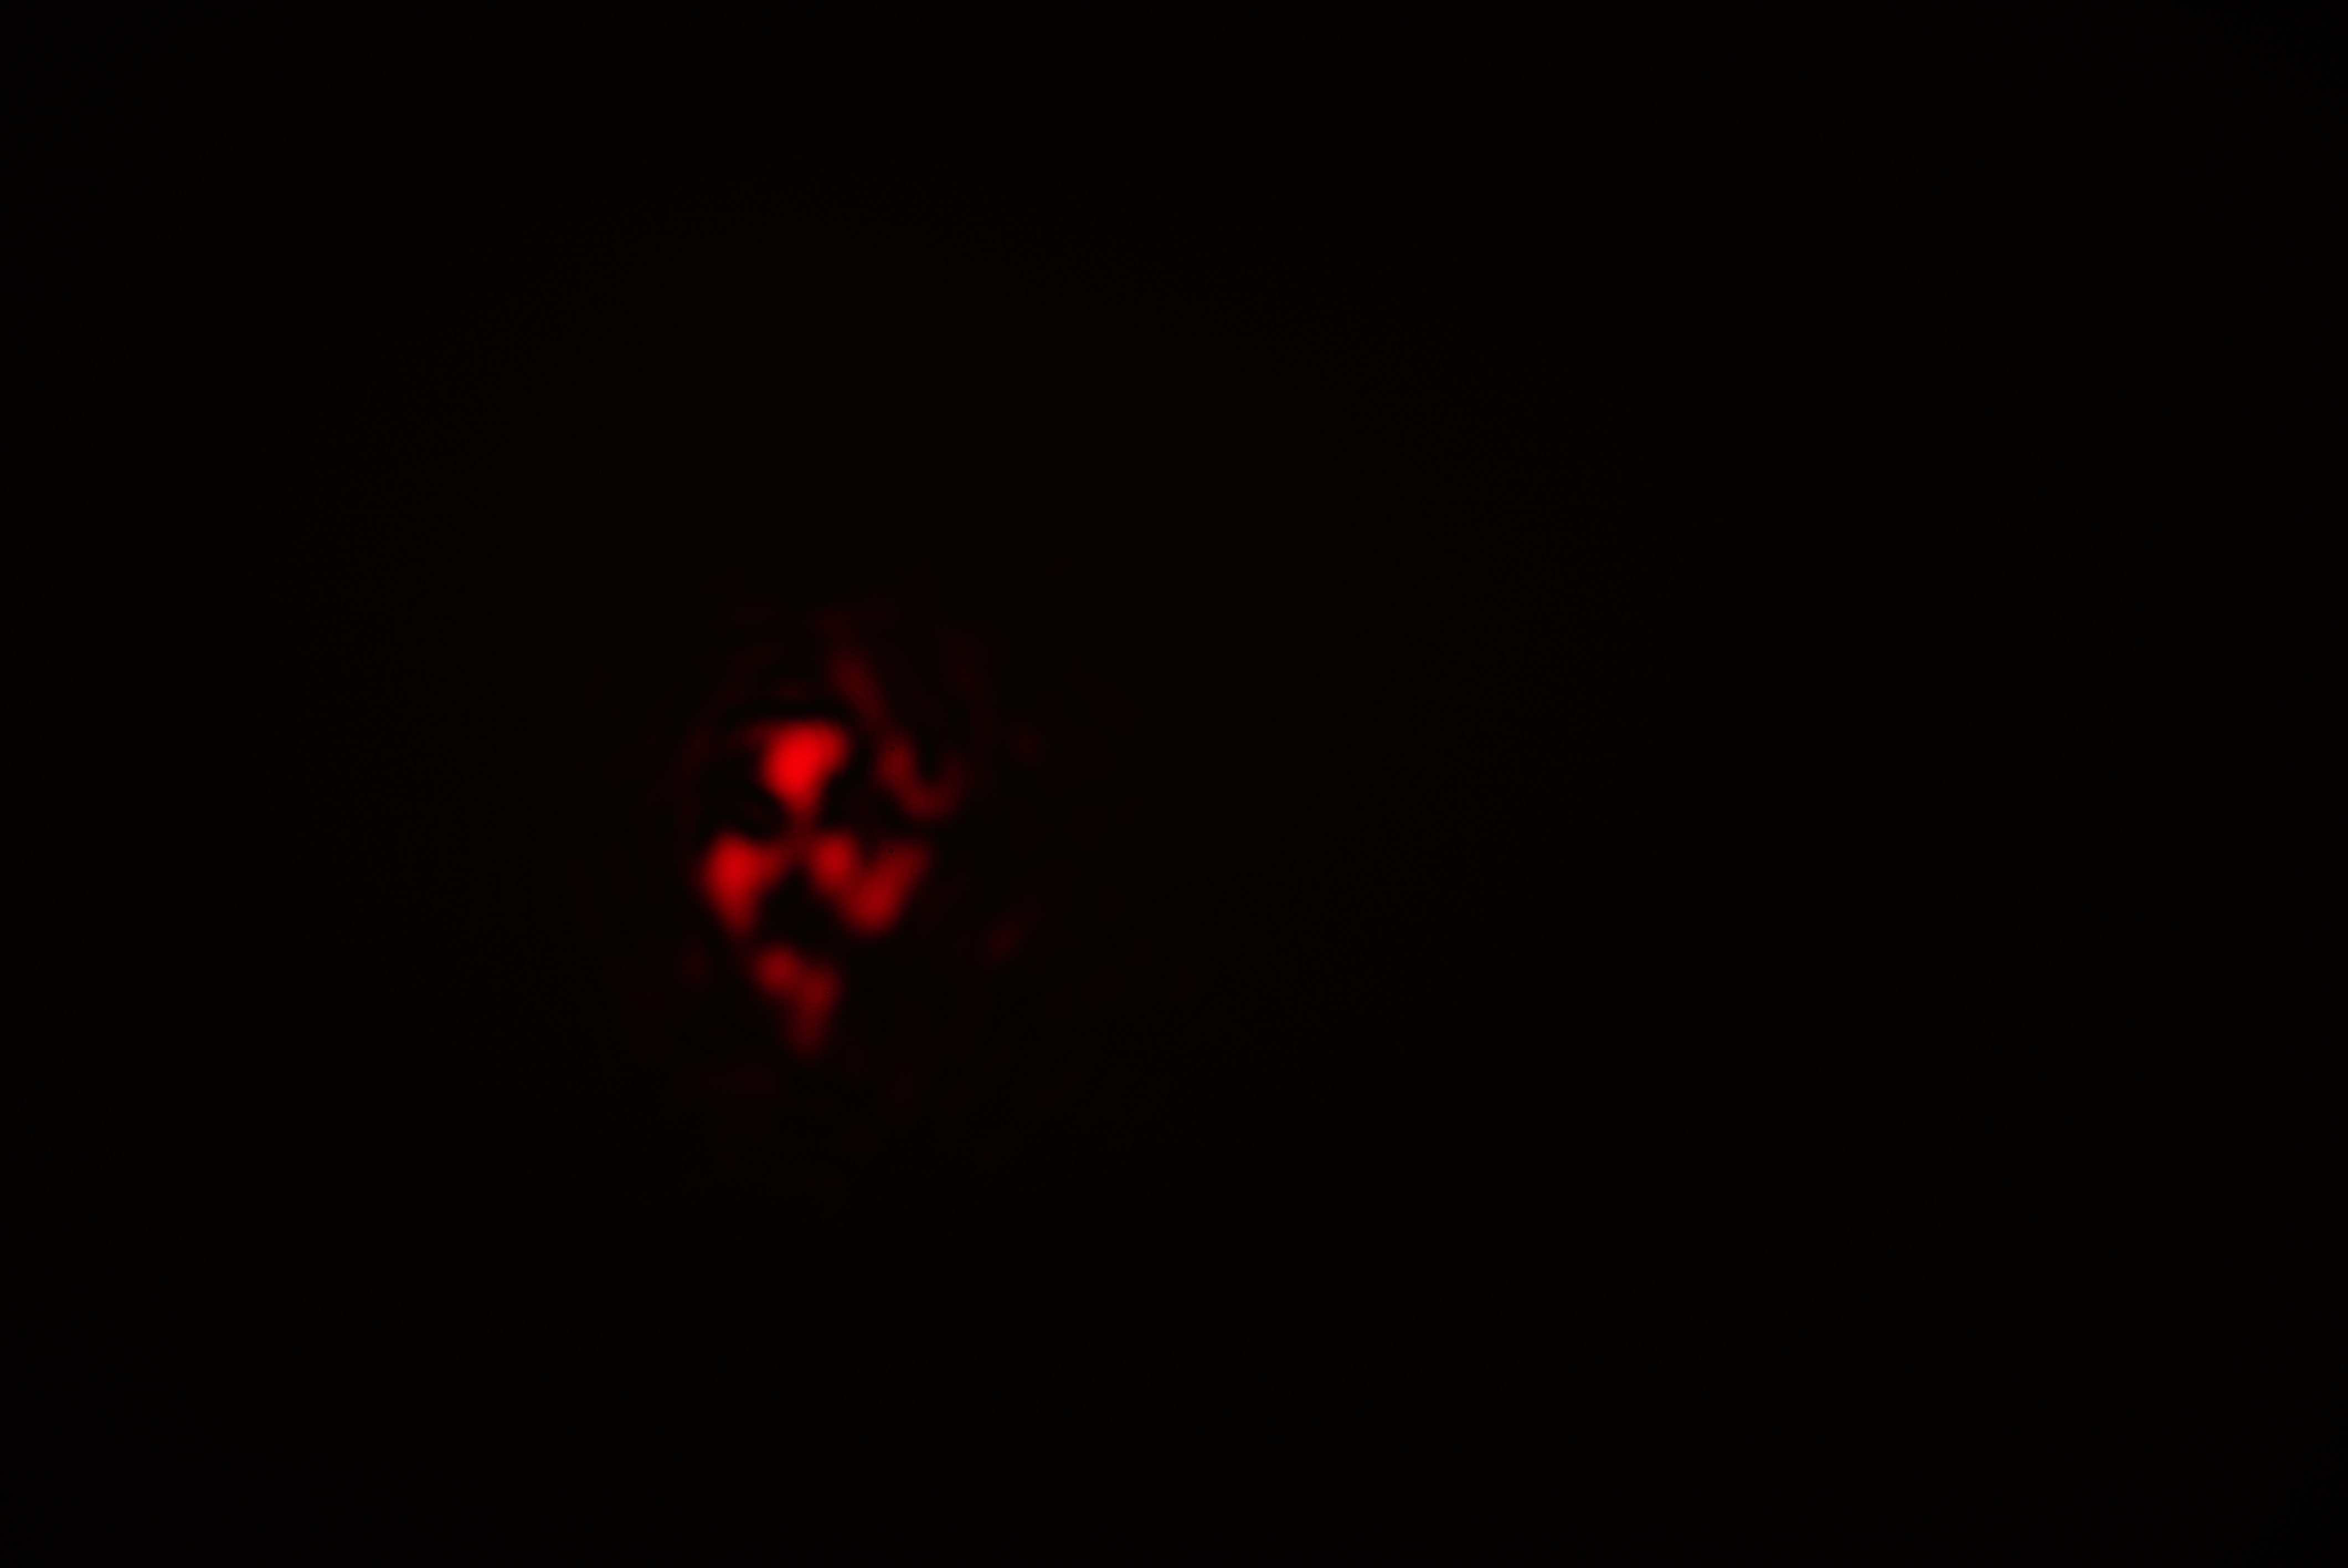
\includegraphics[ width = 0.95 \linewidth ]{figures/AperatureImages/DSC01544.JPG}
        \caption{The captured inverse Fourier transform using the aperture with a diameter of $0.30 \ \si{mm}$}
    \end{minipage}%
\end{figure}